\documentclass[a4,useAMS,usenatbib,usegraphicx,12pt]{article}
%External Packages and personalized macros
%=========================================================================
%		EXTERNAL PACKAGES
%=========================================================================
\usepackage[round]{natbib}
\usepackage[margin=3cm]{geometry}
\usepackage{hyperref}
\usepackage{times}
\usepackage{amsmath} 
\usepackage{amssymb}
\usepackage{graphicx}
\usepackage{array, xcolor, lipsum, bibentry}
\usepackage[nottoc, notlof, notlot]{tocbibind}

\definecolor{lightgray}{gray}{0.8}
\newcolumntype{L}{>{\raggedleft}p{0.14\textwidth}}
\newcolumntype{R}{p{0.8\textwidth}}
\newcommand\VRule{\color{lightgray}\vrule width 0.5pt}

\usepackage{booktabs}% http://ctan.org/pkg/booktabs
\newcommand{\tabitem}{~~\llap{\textbullet}~~}

%=========================================================================
%		INTERNAL MACROS
%=========================================================================
% To highlight comments 
\definecolor{red}{rgb}{1,0.0,0.0}
\newcommand{\red}{\color{red}}
\definecolor{darkgreen}{rgb}{0.0,0.5,0.0}
\newcommand{\SRK}[1]{\textcolor{darkgreen}{\bf SRK: \textit{#1}}}
\newcommand{\SRKED}[1]{\textcolor{darkgreen}{\bf #1}}

\newcommand{\LCDM}{$\Lambda$CDM~}
\newcommand{\beq}{\begin{eqnarray}}  
\newcommand{\eeq}{\end{eqnarray}}  
\newcommand{\zz}{$z\sim 3$} 
\newcommand{\apj}{ApJ}  
\newcommand{\apjs}{ApJS}  
\newcommand{\apjl}{ApJL}  
\newcommand{\aj}{AJ}  
\newcommand{\mnras}{MNRAS}  
\newcommand{\mnrassub}{MNRAS accepted}  
\newcommand{\aap}{A\&A}  
\newcommand{\aaps}{A\&AS}  
\newcommand{\araa}{ARA\&A}  
\newcommand{\nat}{Nature}  
\newcommand{\physrep}{PhR}
\newcommand{\pasp}{PASP}    
\newcommand{\pasj}{PASJ}    
\newcommand{\avg}[1]{\langle{#1}\rangle}  
\newcommand{\ly}{{\ifmmode{{\rm Ly}\alpha}\else{Ly$\alpha$}\fi}}
\newcommand{\hMpc}{{\ifmmode{h^{-1}{\rm Mpc}}\else{$h^{-1}$Mpc }\fi}}  
\newcommand{\hGpc}{{\ifmmode{h^{-1}{\rm Gpc}}\else{$h^{-1}$Gpc }\fi}}  
\newcommand{\hmpc}{{\ifmmode{h^{-1}{\rm Mpc}}\else{$h^{-1}$Mpc }\fi}}  
\newcommand{\hkpc}{{\ifmmode{h^{-1}{\rm kpc}}\else{$h^{-1}$kpc }\fi}}  
\newcommand{\hMsun}{{\ifmmode{h^{-1}{\rm {M_{\odot}}}}\else{$h^{-1}{\rm{M_{\odot}}}$}\fi}}  
\newcommand{\hmsun}{{\ifmmode{h^{-1}{\rm {M_{\odot}}}}\else{$h^{-1}{\rm{M_{\odot}}}$}\fi}}  
\newcommand{\Msun}{{\ifmmode{{\rm {M_{\odot}}}}\else{${\rm{M_{\odot}}}$}\fi}}  
\newcommand{\msun}{{\ifmmode{{\rm {M_{\odot}}}}\else{${\rm{M_{\odot}}}$}\fi}}  
\newcommand{\lya}{{Lyman$\alpha$~}}
\newcommand{\clara}{{\texttt{CLARA}}~}
\newcommand{\rand}{{\ifmmode{{\mathcal{R}}}\else{${\mathcal{R}}$ }\fi}}  


%MY COMMANDS #############################################################
\newcommand{\sub}[1]{\mbox{\scriptsize{#1}}}
\newcommand{\dtot}[2]{ \frac{ d #1 }{d #2} }
\newcommand{\dpar}[2]{ \frac{ \partial #1 }{\partial #2} }
\newcommand{\pr}[1]{ \left( #1 \right) }
\newcommand{\corc}[1]{ \left[ #1 \right] }
\newcommand{\lla}[1]{ \left\{ #1 \right\} }
\newcommand{\bds}[1]{\boldsymbol{ #1 }}
\newcommand{\oiint}{\displaystyle\bigcirc\!\!\!\!\!\!\!\!\int\!\!\!\!\!\int}
\newcommand{\mathsize}[2]{\mbox{\fontsize{#1}{#1}\selectfont $#2$}}
\newcommand{\eq}[2]{\begin{equation} \label{eq:#1} #2 \end{equation}}
\newcommand{\lth}{$\lambda_{th}$ }
%#########################################################################

\setlength\parindent{0pt}
 
\title{{\textbf{Research Proposal for DAAD PhD scholarship}}\\ The Gaseous Cosmic Web with AREPO\\ \color{black}\rule{15cm}{0.5mm}}
\author{Sebastian Bustamante Jaramillo}
\date{}
  
\begin{document}
\maketitle
\begin{center}
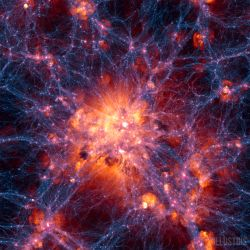
\includegraphics[trim = 0mm 3.5cm 0mm 3.0cm, clip, keepaspectratio=true,
width=0.7\textheight]{Presentation1.png}
\tiny{A projection of the cosmic web in the ILLUSTRIS simulation, that was made 
with AREPO (http://www.illustris-project.org/)}
\end{center}
\tableofcontents
 
\newpage 

%============================================================================== 
\section{General Information}
\small
\subsection*{Information of the Applicant}
\begin{tabular}{L!{\VRule}R}
\bf Name		& Sebastian Bustamante Jaramillo\\
\bf Degree		& B.Sc. in Physics, Universidad de Antioquia (2013)\\
\bf Position	& Adjunct Professor, Universidad de Antioquia\\
\bf Birthday	& { 20$^{th}$ June, 1990}\\
\bf Nationality & Colombian\\
\bf ID			& C.C. 1128400433\\
\bf Address 1	& Avenida 21 \# 57 AA 65, Bello - Colombia (personal)\\
\bf Address 2	& Calle 67 \# 53 - 108, Off. 5-330, Medellin, Colombia (work)\\
\bf Phone		& +057 (4) 4820138\\
\bf Mobile		& +057 3108992409\\
\bf E-mail 1	& macsebas33 \textit{at} gmail.com (personal)\\
\bf E-mail 2	& sebastian.bustamante \textit{at} udea.edu.co (academic)\\
\end{tabular}

\vspace{10pt}

More detailed information of the applicant can be found here \url{http://goo.gl/BPZGzK}

\vspace{15pt}  

\subsection*{Information of the Project}
\begin{tabular}{L!{\VRule}R}
\bf Title		& \bf The Gaseous Cosmic Web with AREPO\\
\bf Field		& Cosmology, Astrophysics, Physical Sciences \\
\bf Advisor 1	& Volker Springel, PhD. Heidelberg Institute for Theoretical Studies (HITS) \& University of Heidelberg, Germany \\
\bf Advisor 2	& Jaime Forero-Romero, PhD. Universidad de los Andes, Colombia \\
\bf University	& University of Heidelberg, IMPRS PhD program \\
\bf Time Frame	& 3 years \\
\end{tabular}
\normalsize
%==============================================================================

\newpage

%==============================================================================
\section{Introduction}


The filamentary nature of the large-scale matter distribution (the so-called 
cosmic web) is one of the most striking features of Universe, being an 
essential part of the current standard paradigm in cosmology. Last generation 
galaxy redshift surveys, such as the \textit{two-degree-Field Galaxy Redshift 
Survey} (2dFGRS, see \citet{Colless03}) and the \textit{Sloan Digital Sky 
Survey} (SDSS, see \citet{Abazajian09}), reveal the cosmic web at a level of 
detail never seen before. In addition, other observational probes like X-ray 
emissions from distant quasars, the Ly-$\alpha$ forest, and weak gravitational 
lensing have also validated this picture undoubtedly.

\

On the theoretical side, early descriptions of the evolution of the large-scale
Universe, based on gravitational instabilities in primordial stages and leaded 
by the seminal work of \citet{Zeldovich70}, predict the cosmic web picture 
\citep{Bond96}. Since then, our understanding of the structure and dynamics of 
the cosmic web has been dramatically improved as new and more powerful 
theoretical and computational tools and better observational data become 
available. In particular, N-body simulations, fuelled by last generation 
computing systems and ever more efficient numerical algorithms, have an 
increasingly important role in revealing the complexity of the large-scale 
Universe.

\

In the $\Lambda$CDM cosmological model there are two different types of 
matter, i.e. the baryonic or luminous matter, corresponding to what we can see, 
and the poorly interacting (and of a still unknown nature) dark matter. The 
current measured abundances indicate a proportion approximately of 6 to 1 
between dark and baryonic matter \citep{Planck13XVI}. Accordingly, most of the 
related numerical research has been made based on dark matter-only N-body 
simulations, where the gas dynamics has been neglected. Nevertheless, recent
studies in filamentary gas accretion in high redsfhit galaxies based on 
simulations \citep{Dekel09} and 

\


. On the other hand, the highly complex \textit{gastrophysical} 
processes involved in baryonic dynamics, i.e. shock heating, photoionization, 
supernova feedback, stellar wind, radiative cooling, star formation and others, 
make extremely difficult to obtain a completely consistent and reliable scenario 
from numerical simulations as many of these processes are not fully understood 
yet. 
Although this duality between observations and simulations can be thought as a 
complementary situation, actually it also makes quite hard to splice both, 
observational data and numerical predictions.

\

Despite the fact that most of above-mentioned \textit{gastrophysical} processes
occurring in baryonic dynamics do represent a challenge for any endeavour for 
simulating the large-scale Universe, the solely hydrodynamic nature of the gas
has been challenging enough even for the most simplified models. Traditionally,
two different hydro-solvers have been used for astrophysical and cosmological 
applications, i.e. a Lagrangian \textit{Smoothed Particle Hydrodynamics} 
(\texttt{SPH}) technique \citep{Monaghan92} (see e.g. the \texttt{GADGET} code, 
\citet{Springel05}) and an Eulerian solver on a mesh with \textit{Adaptive Mesh 
Refinement} (\texttt{AMR}) \citep{Berger89} (see e.g. the \texttt{RAMSES} code, 
\citet{Teyssier02}). \texttt{SPH} is easily implemented on a computer and due to 
its Lagrangian character, its usage is very suitable for many problems as the 
mesh follows the evolution of each single particle, with an continuously 
auto-adjusting resolution. However its same Lagrangian nature causes an 
inhomogeneous and distorted spatial resolution in simulations. This fact makes 
difficult to account for properties of voids in cosmological simulations and also 
causes suppressions in fluid instabilities, making this scheme poor suitable for 
capturing shock dynamics. An artificial viscosity is usually implemented for 
improving the accuracy in these situations. On the other hand, \texttt{AMR} is 
more efficient for capturing shock dynamics without any artificial term, however 
due to the conservative nature of the hydrodynamical equations, a fixed mesh causes 
a lack of Galilean invariance, making the computer implementation considerable 
harder than \texttt{SPH}. Furthermore, due to the unsmooth sampling of physical 
properties, spurious vorticity is introduced to the fluid, making the scheme 
unsuitable for studying turbulent flows (for a further discussion and 
comparison of both schemes, see \citet{Plewa01}).

\

Recently, a completely new paradigm was introduced by \citet{Springel10} that
combines the strengths of \texttt{AMR} and \texttt{SPH} but overcoming their 
weaknesses, i.e. the \texttt{AREPO} code. This code is based on moving mesh 
built from a Voronoi tessellation defined over a set of discrete particles that 
represents the fluid. This procedure is highly efficient as the geometry of the 
mesh follows very closely that of the point distribution, avoiding in this way 
a distorted spatial resolution, but still retaining the auto-adaptivity inherent 
of the \texttt{SPH} scheme. Unlike \texttt{AMR}, the hydro-solver of 
\texttt{AREPO} is based on a Gudonov's scheme that guarantee the Galilean 
invariance and the conservative nature of the solutions. All of these features
makes \texttt{AREPO} highly efficient and accurate for almost any hydrodynamical
problem, including shock dynamics as well as fluid instabilities and turbulent 
flows, essential processes for simulating the high complexity of large-scale 
structure of the Universe. Computationally speaking, \texttt{AREPO} is 
considerably time-consuming due to the high 



%==============================================================================

\newpage
%==============================================================================
\section{Objectives}
%==============================================================================


\begin{itemize}

\item[\checkmark] Understanding, at the light of the last generation \texttt{AREPO} 
simulations, how is the dynamics of the baryonic matter component throughout
the pipeline set up by the potential wells of the dark matter cosmic web.

\item[\checkmark] Quantifying gaseous environmental effects on galaxy formation
and dynamics.

\item[\checkmark] Comparing our results with current (predicting new) observables 
and imprints of the gaseous cosmic web.


\end{itemize}



%==============================================================================
\section{Methodology}
%==============================================================================


The proposed project is subject to a PhD study and will cover the following 
aspects:

\

\begin{itemize}

\item[\checkmark] \textit{First, a set of simulations must be established for 
all succeeding steps. This may involve making new hydrodynamical simulations or
adopting existing ones based on the \texttt{AREPO} code. This also includes a 
complete analysis of the simulations, i.e. characterization of physical fields 
(density, temperature, entropy), construction and analysis of catalogues of 
haloes, and others.}

\end{itemize}

As this project will be almost entirely based on numerical results, 
establishing a set of precise hydrodynamical simulations as a solid base for 
all our succeeding studies is indeed one of the key steps that must be 
fulfilled. The unprecedented accuracy and convergence achieved by the 
\texttt{AREPO} code regarding other traditionally used schemes, will guarantee 
the needed precision.


In Heidelberg, the required computer facilities and the access to the private 
code \texttt{AREPO} (of which Prof. Volker Springel is the main author) is 
granted. Moreover, the renowned research trajectory of Prof. Springel in 
numerical cosmology is certainly another appealing for pursuing this specific 
PhD project.

\

\begin{itemize}

\item[\checkmark] \textit{Second, a preliminary exploration of the dark matter
cosmic web should be done. For this purpose, it is necessary an adaptation of 
some commonly used web-finding schemes (e.g. the V-web and the T-web) to the 
new Voronoi-based paradigm established by the \texttt{AREPO} code.}

\end{itemize}


A first exploration of the structures of the simulations should be done. For
this purpose, many different schemes can be found in the literature, 
but taking into account the reported success of tensor-based 
web-finding schemes (e.g. the V-web and the T-web), in which prof. Jaime 
Forero-Romero has a wide research trajectory, it is quite interesting to 
quantify the dark matter cosmic web of last generation simulations at the light
of them. Nevertheless, it is also necessary to adapt these schemes to the 
Voronoi-based paradigm leaded by \texttt{AREPO} as they was originally intended 
for more traditional \textit{Cloud-in-Cell} methods for estimating the density 
field. It is also worth mentioning previous research experiences of the 
applicant in this topic.

\

\begin{itemize}

\item[\checkmark] \textit{Third, once established the underlying dark matter 
cosmic web, it is necessary to quantify the through gas dynamics. To this aim, 
inward and outward gas flows through potential wells (set by non-linear 
structures such as clusters and filaments) and accretion rates of the gas 
component residing within dark matter halos at different redshifts should be 
computed. At this point, it should be possible to evaluate environmental
influences on different astrophysical phenomena. }

\end{itemize}


In order to exploit the new accuracy provided by the \texttt{AREPO} code, a 
correct quantification of the gas dynamics should be done. The current 
cosmological paradigm predicts a complex pipeline set by the potential well of 
non-linear structures, generally corresponding to clusters and filaments, 
through which the gas is transported toward over-dense regions like dark matter 
haloes. This process yields to different environmental phenomena of great current 
interest. We list here the most relevant for this project: influence of 
filament-induced flows on star forming galaxies at high redshifts, acquisition of 
the spin of galaxies through exchanging of angular momentum with the gaseous 
cosmic web, and kinematical and dynamical effects of the host environment on Local 
Group-like systems.

\

\begin{itemize}

\item[\checkmark] \textit{Finally, a detailed comparison of our potential 
predictions (or restrictions) with currently available observational data
should be done.}

\end{itemize}



%==============================================================================
\section{Current State}
%==============================================================================


At present, the applicant has already the fundamental basis in Astrophysics and
Cosmology required for this investigation. This can be confirmed by his research 
trajectory, including a paper (as co-author) published in \textit{ApJL} in which 
was studied the kinematics of the Local Group in a cosmological context, and some
participations in academic congresses. Furthermore, a Bachelor's thesis
\footnote{Further information and an electronic version of this 
thesis can be found here \url{https://github.com/sbustamante/Thesis}.}, where was 
numerically studied the preferred place of Local Group-like systems regarding the 
host environment in the cosmic web, also proves the ability of the applicant for
handling simulations and massive data, a skill that is indeed necessary for 
carrying out this project.


%==============================================================================
\section{Timetable}
%==============================================================================

\begin{table}[h]
\begin{flushleft}
\begin{center}
  \begin{tabular}{l  l} \hline\hline
	\centering\textbf{Year} & \textbf{Goals} \\ \hline
	%First year
	First  
	& \tabitem First goal \\
	& \tabitem Second goal\\
	
	\\
	%Second year	
	Second
	& \tabitem First goal \\
	& \tabitem Second goal\\

	\\	
	%Third year	
	Third
	& \tabitem First goal \\
	& \tabitem Second goal\\ 
	
	\hline\hline
  \end{tabular}  
\end{center}
\end{flushleft}
\end{table}


%==============================================================================
\bibliographystyle{latex/mn2e}
\renewcommand{\bibname}{8\ \ \ \ Bibliography}
\bibliography{references.bib}
%==============================================================================



\end{document}